\subsection*{Noninteracting Fermions}

Consider Hamiltonian
\begin{equation*}
	H = \sum_{n, \sigma} c_{k \sigma}\D (\varepsilon_k - \mu) c_{k\sigma} = \sum_{k, \sigma} \xi_k c_{ka}\D c_{k \sigma},
\end{equation*}
with $T=0$ 
\begin{equation*}
	\gs = \prod_{|k| < \kF} c_{k \sigma}\D \ket{0}.
\end{equation*}
% \textbf{Single-particle exitation}. 
And we know very well single-particle exitations. Let's add a pericle $k > \kF$
\begin{equation*}
	\delta E_k = \frac{1}{2m}\left(k^2 - \kF^2\right) = \frac{1}{2m} \left(
		(\kF + \delta k)^2 - \kF^2
	\right) \approx \vF \cdot \delta k.
\end{equation*}
with $\delta k = |k-\kF| \ll \kF$ and $\vF = \kF / m$. If we remove a particle $k < \kF$ 
\begin{equation*}
	\delta E_k = \frac{1}{2m}\left(\kF^2 - (\kF - \delta k)^2\right) = \vF \cdot \delta k.
\end{equation*}
We could define Wilson ration as
\begin{equation*}
	R_W = \frac{\pi^2 \kB^2}{3 \muB^2} \frac{\chi}{\gamma} = 1,
\end{equation*}
for free fermions despite the band structure. 

\begin{figure}[h]
    \centering
    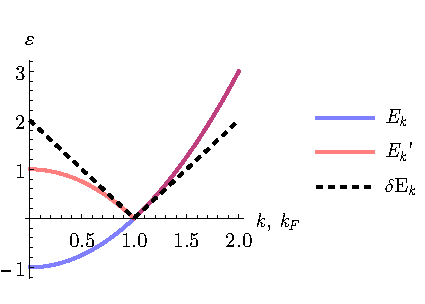
\includegraphics{imgs/FS.pdf}
    \caption{Single-particle exitations}
    \label{fig:1}
\end{figure}

% \textbf{Two-particle exitation}. It looks like
% \begin{equation*}
% 	c_{k+q}\D c_k \gs
% \end{equation*}

